\begin{knitrout}
\definecolor{shadecolor}{rgb}{0.969, 0.969, 0.969}\color{fgcolor}\begin{kframe}
\begin{alltt}
\hlkwd{library}\hlstd{(knitr)}
\hlkwd{Sweave2knitr}\hlstd{(}\hlstr{'sweaveEx.Rnw'}\hlstd{)}
\end{alltt}


{\ttfamily\noindent\itshape\color{messagecolor}{\#\# removing the unnecessary option fig=TRUE:\\\#\#\ \ \ \  * test2, fig=TRUE\\\#\#\ \ \ \  * test3, fig=TRUE, height=4, width=6}}

{\ttfamily\noindent\itshape\color{messagecolor}{\#\# replacing results=tex with results=asis:\\\#\#\ \ \ \  * manualtab, results=tex,echo=FALSE\\\#\#\ \ \ \  * xtable1, results=tex\\\#\#\ \ \ \  * xtable2, results=tex}}

{\ttfamily\noindent\itshape\color{messagecolor}{\#\# quoting the results option:\\\#\#\ \ \ \  * manualtab, results=asis,echo=FALSE\\\#\#\ \ \ \  * xtable1, results=asis\\\#\#\ \ \ \  * xtable2, results=asis}}

{\ttfamily\noindent\itshape\color{messagecolor}{\#\# replacing width/height with fig.width/fig.height:\\\#\#\ \ \ \  * test3, , height=4, width=6}}

{\ttfamily\noindent\itshape\color{messagecolor}{\#\# replacing prefix.string=foo with fig.path='foo':\\\#\#\ \ \ \  * prefix.string=Fig}}

{\ttfamily\noindent\itshape\color{messagecolor}{\#\# changing \textbackslash{}SweaveOpts\{\} to opts\_chunk\$set():\\\#\#\ \ \ \  * \textbackslash{}SweaveOpts\{highlight=TRUE, tidy=TRUE, keep.space=TRUE,\\\#\#\ \ \ \ \ \  keep.blank.space=FALSE, keep.comment=TRUE\}\\\#\#\ \ \ \  * \textbackslash{}SweaveOpts\{prefix.string=Fig\}}}\end{kframe}
\end{knitrout}
\documentclass{article}
\usepackage{graphicx}
\usepackage{hyperref}
\usepackage{amsmath}
\usepackage{times}

\textwidth=6.2in
\textheight=8.5in
%\parskip=.3cm
\oddsidemargin=.1in
\evensidemargin=.1in
\headheight=-.3in


%------------------------------------------------------------
% newcommand
%------------------------------------------------------------
\newcommand{\scscst}{\scriptscriptstyle}
\newcommand{\scst}{\scriptstyle}
\newcommand{\Robject}[1]{{\texttt{#1}}}
\newcommand{\Rfunction}[1]{{\texttt{#1}}}
\newcommand{\Rclass}[1]{\textit{#1}}
\newcommand{\Rpackage}[1]{\textit{#1}}
\newcommand{\Rexpression}[1]{\texttt{#1}}
\newcommand{\Rmethod}[1]{{\texttt{#1}}}
\newcommand{\Rfunarg}[1]{{\texttt{#1}}}

\begin{document}

%------------------------------------------------------------
\title{Simple example of Sweave}
%------------------------------------------------------------
\author{Aedin Culhane}
%\date{}

\SweaveOpts{highlight=TRUE, tidy=TRUE, keep.space=TRUE, keep.blank.space=FALSE, keep.comment=TRUE}
\SweaveOpts{prefix.string=Fig}


\maketitle
\tableofcontents


%-------------------------------------------
\section{Introduction}
%--------------------------------------------

Just a simple introduction to Sweave. 

\begin{knitrout}
\definecolor{shadecolor}{rgb}{0.969, 0.969, 0.969}\color{fgcolor}\begin{kframe}
\begin{alltt}
\hlstd{a}\hlkwb{=}\hlnum{1}
\hlstd{b}\hlkwb{=}\hlnum{4}
\hlstd{a}\hlopt{+}\hlstd{b}
\end{alltt}
\begin{verbatim}
## [1] 5
\end{verbatim}
\begin{alltt}
\hlkwd{print}\hlstd{(}\hlstr{"hello"}\hlstd{)}
\end{alltt}
\begin{verbatim}
## [1] "hello"
\end{verbatim}
\end{kframe}
\end{knitrout}

We can call R commands from the text. For example a+b= 5

%-------------------------------------------
\section{Including a Plot}
%--------------------------------------------
Now for a plot.  Note we include fig=TRUE, which prints the plot within the document


\begin{knitrout}
\definecolor{shadecolor}{rgb}{0.969, 0.969, 0.969}\color{fgcolor}\begin{kframe}
\begin{alltt}
\hlkwd{plot}\hlstd{(}\hlnum{1}\hlopt{:}\hlnum{10}\hlstd{,} \hlkwc{col}\hlstd{=}\hlstr{"red"}\hlstd{,} \hlkwc{pch}\hlstd{=}\hlnum{19}\hlstd{)}
\end{alltt}
\end{kframe}
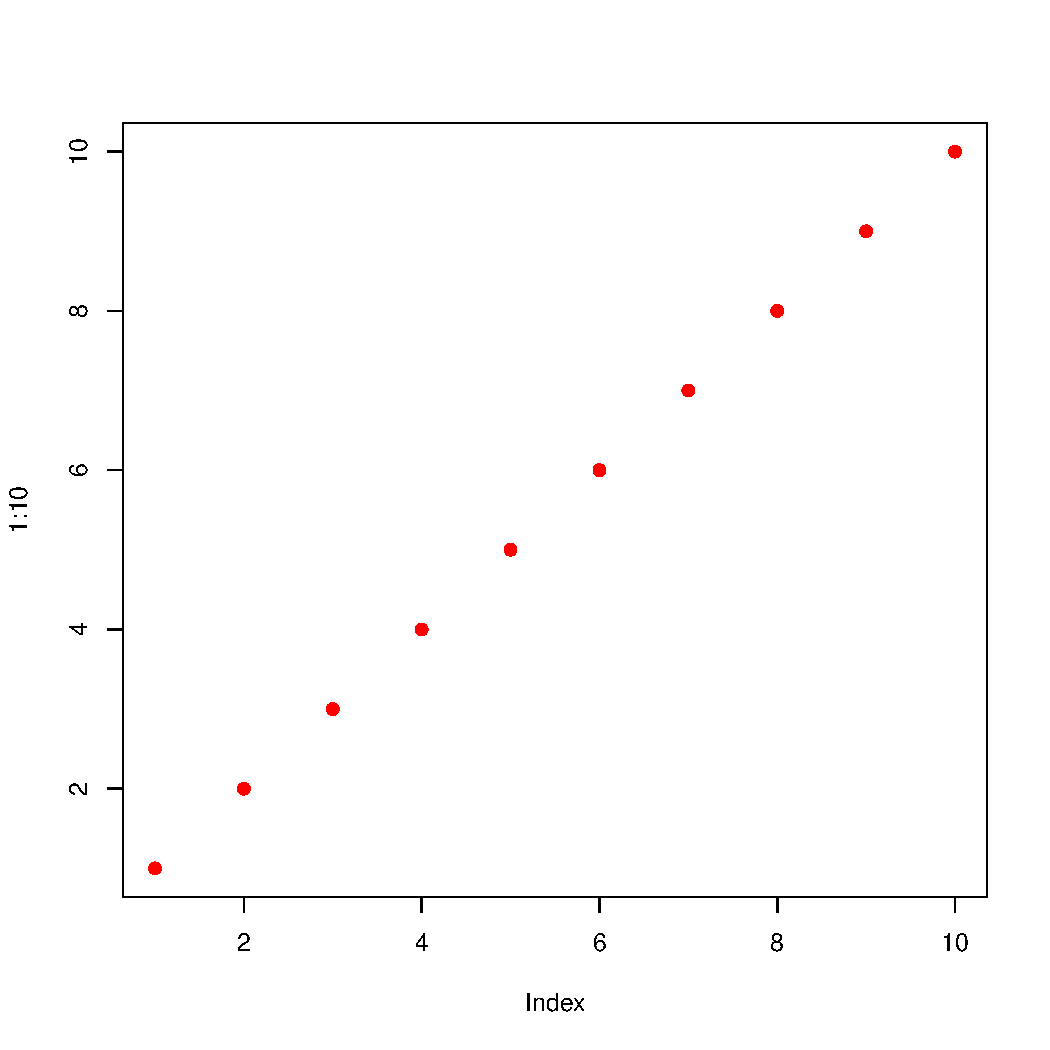
\includegraphics[width=\maxwidth]{figure/test2-1} 

\end{knitrout}

Thats it.... simple hey!


%------------------------------------
\subsection{More on Plots}
%-------------------------------------

To make the plot a little nicer, we can add a caption. Also lets change the size of the plot to be 4" in height and 6" in width

\begin{figure}
\begin{knitrout}
\definecolor{shadecolor}{rgb}{0.969, 0.969, 0.969}\color{fgcolor}\begin{kframe}
\begin{alltt}
\hlkwd{par}\hlstd{(}\hlkwc{mfrow}\hlstd{=}\hlkwd{c}\hlstd{(}\hlnum{1}\hlstd{,}\hlnum{2}\hlstd{))}
\hlkwd{plot}\hlstd{(}\hlnum{1}\hlopt{:}\hlnum{10}\hlstd{,} \hlkwc{col}\hlstd{=}\hlstr{"green"}\hlstd{,} \hlkwc{pch}\hlstd{=}\hlnum{21}\hlstd{)}
\hlkwd{barplot}\hlstd{(}\hlkwc{height}\hlstd{=}\hlkwd{sample}\hlstd{(}\hlnum{1}\hlopt{:}\hlnum{10}\hlstd{,}\hlnum{5}\hlstd{),} \hlkwc{names}\hlstd{=LETTERS[}\hlnum{1}\hlopt{:}\hlnum{5}\hlstd{],} \hlkwc{col}\hlstd{=}\hlnum{1}\hlopt{:}\hlnum{5}\hlstd{)}
\end{alltt}
\end{kframe}
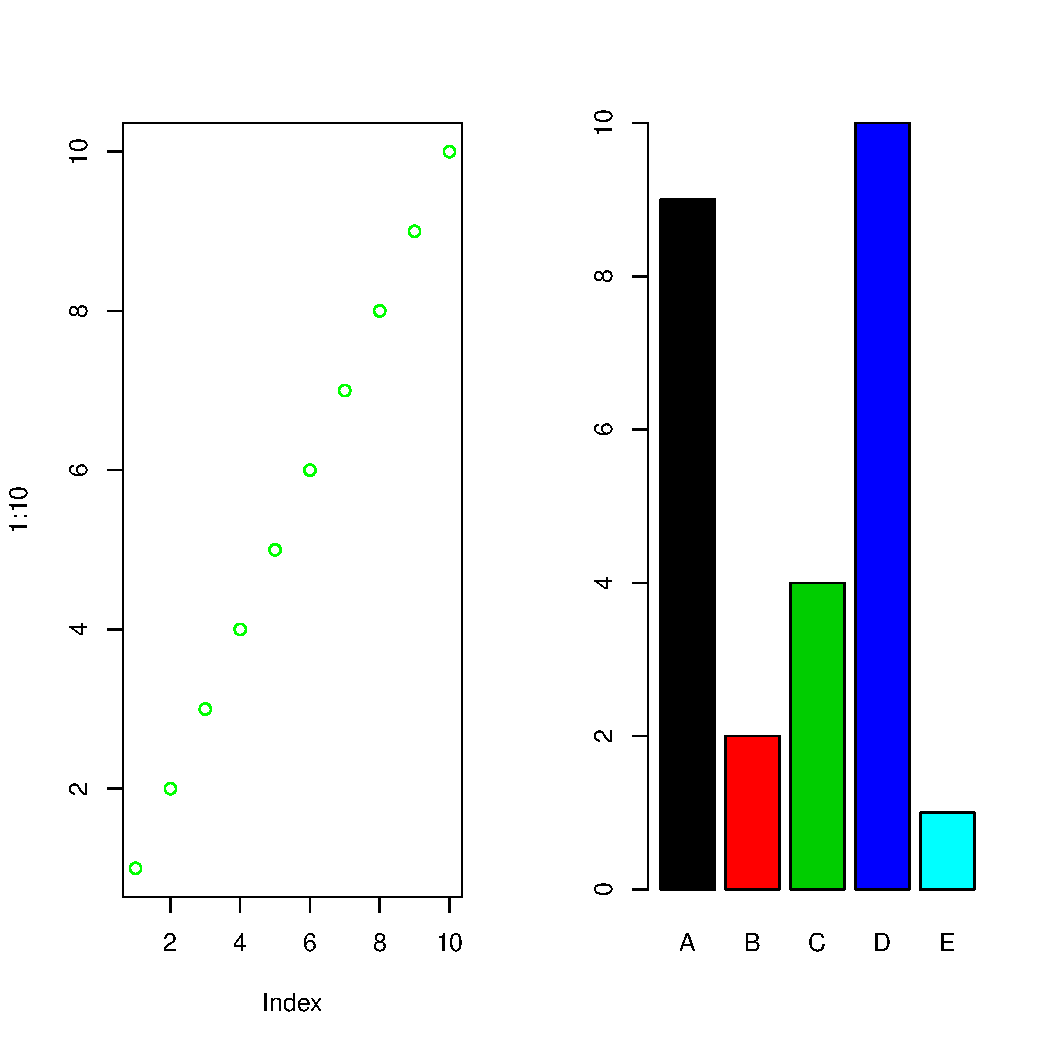
\includegraphics[width=\maxwidth]{figure/test3-1} 

\end{knitrout}

\caption{Plot of 1:10 and a bar plot beside it in a figure that is 4x6 inches}

\end{figure}

\newpage
%------------------------------------
\subsection{Creating a table}
%-------------------------------------

Lets include a table using the dataset,  which is included in the default core installation of R. It contains the height and weight of 15 women.

\begin{knitrout}
\definecolor{shadecolor}{rgb}{0.969, 0.969, 0.969}\color{fgcolor}\begin{kframe}
\begin{alltt}
\hlkwd{require}\hlstd{(xtable)}
\end{alltt}


{\ttfamily\noindent\itshape\color{messagecolor}{\#\# Loading required package: xtable}}\begin{alltt}
\hlstd{myTable}\hlkwb{<-}\hlkwd{summary}\hlstd{(women)}
\end{alltt}
\end{kframe}
\end{knitrout}

We can manually encode a table in latex 


\begin{center}
\begin{tabular}{rrrrrrrr} 









